\documentclass[11pt]{article}

\usepackage{float}
% NOTE: Add in the relevant information to the commands below; or, if you'll be using the same information frequently, add these commands at the top of paolo-pset.tex file. 
\newcommand{\name}{Agustin Esteva}
\newcommand{\email}{aesteva@uchicago.edu}
\newcommand{\classnum}{13210}
\newcommand{\subject}{SSI: Formal Theory}
\newcommand{\instructors}{Scott Gehlbach}
\newcommand{\assignment}{Problem Set 4}
\newcommand{\semester}{Winter 2024}
\newcommand{\duedate}{2024-02-03}
\newcommand{\bA}{\mathbf{A}}
\newcommand{\bB}{\mathbf{B}}
\newcommand{\bC}{\mathbf{C}}
\newcommand{\bD}{\mathbf{D}}
\newcommand{\bE}{\mathbf{E}}
\newcommand{\bF}{\mathbf{F}}
\newcommand{\bG}{\mathbf{G}}
\newcommand{\bH}{\mathbf{H}}
\newcommand{\bI}{\mathbf{I}}
\newcommand{\bJ}{\mathbf{J}}
\newcommand{\bK}{\mathbf{K}}
\newcommand{\bL}{\mathbf{L}}
\newcommand{\bM}{\mathbf{M}}
\newcommand{\bN}{\mathbf{N}}
\newcommand{\bO}{\mathbf{O}}
\newcommand{\bP}{\mathbf{P}}
\newcommand{\bQ}{\mathbf{Q}}
\newcommand{\bR}{\mathbf{R}}
\newcommand{\bS}{\mathbf{S}}
\newcommand{\bT}{\mathbf{T}}
\newcommand{\bU}{\mathbf{U}}
\newcommand{\bV}{\mathbf{V}}
\newcommand{\bW}{\mathbf{W}}
\newcommand{\bX}{\mathbf{X}}
\newcommand{\bY}{\mathbf{Y}}
\newcommand{\bZ}{\mathbf{Z}}
\newcommand{\Var}{\text{Var}}

%% blackboard bold math capitals
\newcommand{\bbA}{\mathbb{A}}
\newcommand{\bbB}{\mathbb{B}}
\newcommand{\bbC}{\mathbb{C}}
\newcommand{\bbD}{\mathbb{D}}
\newcommand{\bbE}{\mathbb{E}}
\newcommand{\bbF}{\mathbb{F}}
\newcommand{\bbG}{\mathbb{G}}
\newcommand{\bbH}{\mathbb{H}}
\newcommand{\bbI}{\mathbb{I}}
\newcommand{\bbJ}{\mathbb{J}}
\newcommand{\bbK}{\mathbb{K}}
\newcommand{\bbL}{\mathbb{L}}
\newcommand{\bbM}{\mathbb{M}}
\newcommand{\bbN}{\mathbb{N}}
\newcommand{\bbO}{\mathbb{O}}
\newcommand{\bbP}{\mathbb{P}}
\newcommand{\bbQ}{\mathbb{Q}}
\newcommand{\bbR}{\mathbb{R}}
\newcommand{\bbS}{\mathbb{S}}
\newcommand{\bbT}{\mathbb{T}}
\newcommand{\bbU}{\mathbb{U}}
\newcommand{\bbV}{\mathbb{V}}
\newcommand{\bbW}{\mathbb{W}}
\newcommand{\bbX}{\mathbb{X}}
\newcommand{\bbY}{\mathbb{Y}}
\newcommand{\bbZ}{\mathbb{Z}}

%% script math capitals
\newcommand{\sA}{\mathscr{A}}
\newcommand{\sB}{\mathscr{B}}
\newcommand{\sC}{\mathscr{C}}
\newcommand{\sD}{\mathscr{D}}
\newcommand{\sE}{\mathscr{E}}
\newcommand{\sF}{\mathscr{F}}
\newcommand{\sG}{\mathscr{G}}
\newcommand{\sH}{\mathscr{H}}
\newcommand{\sI}{\mathscr{I}}
\newcommand{\sJ}{\mathscr{J}}
\newcommand{\sK}{\mathscr{K}}
\newcommand{\sL}{\mathscr{L}}
\newcommand{\sM}{\mathscr{M}}
\newcommand{\sN}{\mathscr{N}}
\newcommand{\sO}{\mathscr{O}}
\newcommand{\sP}{\mathscr{P}}
\newcommand{\sQ}{\mathscr{Q}}
\newcommand{\sR}{\mathscr{R}}
\newcommand{\sS}{\mathscr{S}}
\newcommand{\sT}{\mathscr{T}}
\newcommand{\sU}{\mathscr{U}}
\newcommand{\sV}{\mathscr{V}}
\newcommand{\sW}{\mathscr{W}}
\newcommand{\sX}{\mathscr{X}}
\newcommand{\sY}{\mathscr{Y}}
\newcommand{\sZ}{\mathscr{Z}}


\renewcommand{\emptyset}{\O}

\newcommand{\abs}[1]{\lvert #1 \rvert}
\newcommand{\norm}[1]{\lVert #1 \rVert}
\newcommand{\sm}{\setminus}


\newcommand{\sarr}{\rightarrow}
\newcommand{\arr}{\longrightarrow}

% NOTE: Defining collaborators is optional; to not list collaborators, comment out the line below.
%\newcommand{\collaborators}{Alyssa P. Hacker (\texttt{aphacker}), Ben Bitdiddle (\texttt{bitdiddle})}

% Copyright 2021 Paolo Adajar (padajar.com, paoloadajar@mit.edu)
% 
% Permission is hereby granted, free of charge, to any person obtaining a copy of this software and associated documentation files (the "Software"), to deal in the Software without restriction, including without limitation the rights to use, copy, modify, merge, publish, distribute, sublicense, and/or sell copies of the Software, and to permit persons to whom the Software is furnished to do so, subject to the following conditions:
%
% The above copyright notice and this permission notice shall be included in all copies or substantial portions of the Software.
% 
% THE SOFTWARE IS PROVIDED "AS IS", WITHOUT WARRANTY OF ANY KIND, EXPRESS OR IMPLIED, INCLUDING BUT NOT LIMITED TO THE WARRANTIES OF MERCHANTABILITY, FITNESS FOR A PARTICULAR PURPOSE AND NONINFRINGEMENT. IN NO EVENT SHALL THE AUTHORS OR COPYRIGHT HOLDERS BE LIABLE FOR ANY CLAIM, DAMAGES OR OTHER LIABILITY, WHETHER IN AN ACTION OF CONTRACT, TORT OR OTHERWISE, ARISING FROM, OUT OF OR IN CONNECTION WITH THE SOFTWARE OR THE USE OR OTHER DEALINGS IN THE SOFTWARE.

\usepackage{fullpage}
\usepackage{enumitem}
\usepackage{amsfonts, amssymb, amsmath,amsthm}
\usepackage{mathtools}
\usepackage[pdftex, pdfauthor={\name}, pdftitle={\classnum~\assignment}]{hyperref}
\usepackage[dvipsnames]{xcolor}
\usepackage{bbm}
\usepackage{graphicx}
\usepackage{mathrsfs}
\usepackage{pdfpages}
\usepackage{tabularx}
\usepackage{pdflscape}
\usepackage{makecell}
\usepackage{booktabs}
\usepackage{natbib}
\usepackage{caption}
\usepackage{subcaption}
\usepackage{physics}
\usepackage[many]{tcolorbox}
\usepackage{version}
\usepackage{ifthen}
\usepackage{cancel}
\usepackage{listings}
\usepackage{courier}

\usepackage{tikz}
\usepackage{istgame}

\hypersetup{
	colorlinks=true,
	linkcolor=blue,
	filecolor=magenta,
	urlcolor=blue,
}

\setlength{\parindent}{0mm}
\setlength{\parskip}{2mm}

\setlist[enumerate]{label=({\alph*})}
\setlist[enumerate, 2]{label=({\roman*})}

\allowdisplaybreaks[1]

\newcommand{\psetheader}{
	\ifthenelse{\isundefined{\collaborators}}{
		\begin{center}
			{\setlength{\parindent}{0cm} \setlength{\parskip}{0mm}
				
				{\textbf{\classnum~\semester:~\assignment} \hfill \name}
				
				\subject \hfill \href{mailto:\email}{\tt \email}
				
				Instructor(s):~\instructors \hfill Due Date:~\duedate	
				
				\hrulefill}
		\end{center}
	}{
		\begin{center}
			{\setlength{\parindent}{0cm} \setlength{\parskip}{0mm}
				
				{\textbf{\classnum~\semester:~\assignment} \hfill \name\footnote{Collaborator(s): \collaborators}}
				
				\subject \hfill \href{mailto:\email}{\tt \email}
				
				Instructor(s):~\instructors \hfill Due Date:~\duedate	
				
				\hrulefill}
		\end{center}
	}
}

\renewcommand{\thepage}{\classnum~\assignment \hfill \arabic{page}}

\makeatletter
\def\points{\@ifnextchar[{\@with}{\@without}}
\def\@with[#1]#2{{\ifthenelse{\equal{#2}{1}}{{[1 point, #1]}}{{[#2 points, #1]}}}}
\def\@without#1{\ifthenelse{\equal{#1}{1}}{{[1 point]}}{{[#1 points]}}}
\makeatother

\newtheoremstyle{theorem-custom}%
{}{}%
{}{}%
{\itshape}{.}%
{ }%
{\thmname{#1}\thmnumber{ #2}\thmnote{ (#3)}}

\theoremstyle{theorem-custom}

\newtheorem{theorem}{Theorem}
\newtheorem{lemma}[theorem]{Lemma}
\newtheorem{example}[theorem]{Example}

\newenvironment{problem}[1]{\color{black} #1}{}

\newenvironment{solution}{%
	\leavevmode\begin{tcolorbox}[breakable, colback=green!5!white,colframe=green!75!black, enhanced jigsaw] \proof[\scshape Solution:] \setlength{\parskip}{2mm}%
	}{\renewcommand{\qedsymbol}{$\blacksquare$} \endproof \end{tcolorbox}}

\newenvironment{reflection}{\begin{tcolorbox}[breakable, colback=black!8!white,colframe=black!60!white, enhanced jigsaw, parbox = false]\textsc{Reflections:}}{\end{tcolorbox}}

\newcommand{\qedh}{\renewcommand{\qedsymbol}{$\blacksquare$}\qedhere}

\definecolor{mygreen}{rgb}{0,0.6,0}
\definecolor{mygray}{rgb}{0.5,0.5,0.5}
\definecolor{mymauve}{rgb}{0.58,0,0.82}

% from https://github.com/satejsoman/stata-lstlisting
% language definition
\lstdefinelanguage{Stata}{
	% System commands
	morekeywords=[1]{regress, reg, summarize, sum, display, di, generate, gen, bysort, use, import, delimited, predict, quietly, probit, margins, test},
	% Reserved words
	morekeywords=[2]{aggregate, array, boolean, break, byte, case, catch, class, colvector, complex, const, continue, default, delegate, delete, do, double, else, eltypedef, end, enum, explicit, export, external, float, for, friend, function, global, goto, if, inline, int, local, long, mata, matrix, namespace, new, numeric, NULL, operator, orgtypedef, pointer, polymorphic, pragma, private, protected, public, quad, real, return, rowvector, scalar, short, signed, static, strL, string, struct, super, switch, template, this, throw, transmorphic, try, typedef, typename, union, unsigned, using, vector, version, virtual, void, volatile, while,},
	% Keywords
	morekeywords=[3]{forvalues, foreach, set},
	% Date and time functions
	morekeywords=[4]{bofd, Cdhms, Chms, Clock, clock, Cmdyhms, Cofc, cofC, Cofd, cofd, daily, date, day, dhms, dofb, dofC, dofc, dofh, dofm, dofq, dofw, dofy, dow, doy, halfyear, halfyearly, hh, hhC, hms, hofd, hours, mdy, mdyhms, minutes, mm, mmC, mofd, month, monthly, msofhours, msofminutes, msofseconds, qofd, quarter, quarterly, seconds, ss, ssC, tC, tc, td, th, tm, tq, tw, week, weekly, wofd, year, yearly, yh, ym, yofd, yq, yw,},
	% Mathematical functions
	morekeywords=[5]{abs, ceil, cloglog, comb, digamma, exp, expm1, floor, int, invcloglog, invlogit, ln, ln1m, ln, ln1p, ln, lnfactorial, lngamma, log, log10, log1m, log1p, logit, max, min, mod, reldif, round, sign, sqrt, sum, trigamma, trunc,},
	% Matrix functions
	morekeywords=[6]{cholesky, coleqnumb, colnfreeparms, colnumb, colsof, corr, det, diag, diag0cnt, el, get, hadamard, I, inv, invsym, issymmetric, J, matmissing, matuniform, mreldif, nullmat, roweqnumb, rownfreeparms, rownumb, rowsof, sweep, trace, vec, vecdiag, },
	% Programming functions
	morekeywords=[7]{autocode, byteorder, c, _caller, chop, abs, clip, cond, e, fileexists, fileread, filereaderror, filewrite, float, fmtwidth, has_eprop, inlist, inrange, irecode, matrix, maxbyte, maxdouble, maxfloat, maxint, maxlong, mi, minbyte, mindouble, minfloat, minint, minlong, missing, r, recode, replay, return, s, scalar, smallestdouble,},
	% Random-number functions
	morekeywords=[8]{rbeta, rbinomial, rcauchy, rchi2, rexponential, rgamma, rhypergeometric, rigaussian, rlaplace, rlogistic, rnbinomial, rnormal, rpoisson, rt, runiform, runiformint, rweibull, rweibullph,},
	% Selecting time-span functions
	morekeywords=[9]{tin, twithin,},
	% Statistical functions
	morekeywords=[10]{betaden, binomial, binomialp, binomialtail, binormal, cauchy, cauchyden, cauchytail, chi2, chi2den, chi2tail, dgammapda, dgammapdada, dgammapdadx, dgammapdx, dgammapdxdx, dunnettprob, exponential, exponentialden, exponentialtail, F, Fden, Ftail, gammaden, gammap, gammaptail, hypergeometric, hypergeometricp, ibeta, ibetatail, igaussian, igaussianden, igaussiantail, invbinomial, invbinomialtail, invcauchy, invcauchytail, invchi2, invchi2tail, invdunnettprob, invexponential, invexponentialtail, invF, invFtail, invgammap, invgammaptail, invibeta, invibetatail, invigaussian, invigaussiantail, invlaplace, invlaplacetail, invlogistic, invlogistictail, invnbinomial, invnbinomialtail, invnchi2, invnF, invnFtail, invnibeta, invnormal, invnt, invnttail, invpoisson, invpoissontail, invt, invttail, invtukeyprob, invweibull, invweibullph, invweibullphtail, invweibulltail, laplace, laplaceden, laplacetail, lncauchyden, lnigammaden, lnigaussianden, lniwishartden, lnlaplaceden, lnmvnormalden, lnnormal, lnnormalden, lnwishartden, logistic, logisticden, logistictail, nbetaden, nbinomial, nbinomialp, nbinomialtail, nchi2, nchi2den, nchi2tail, nF, nFden, nFtail, nibeta, normal, normalden, npnchi2, npnF, npnt, nt, ntden, nttail, poisson, poissonp, poissontail, t, tden, ttail, tukeyprob, weibull, weibullden, weibullph, weibullphden, weibullphtail, weibulltail,},
	% String functions 
	morekeywords=[11]{abbrev, char, collatorlocale, collatorversion, indexnot, plural, plural, real, regexm, regexr, regexs, soundex, soundex_nara, strcat, strdup, string, strofreal, string, strofreal, stritrim, strlen, strlower, strltrim, strmatch, strofreal, strofreal, strpos, strproper, strreverse, strrpos, strrtrim, strtoname, strtrim, strupper, subinstr, subinword, substr, tobytes, uchar, udstrlen, udsubstr, uisdigit, uisletter, ustrcompare, ustrcompareex, ustrfix, ustrfrom, ustrinvalidcnt, ustrleft, ustrlen, ustrlower, ustrltrim, ustrnormalize, ustrpos, ustrregexm, ustrregexra, ustrregexrf, ustrregexs, ustrreverse, ustrright, ustrrpos, ustrrtrim, ustrsortkey, ustrsortkeyex, ustrtitle, ustrto, ustrtohex, ustrtoname, ustrtrim, ustrunescape, ustrupper, ustrword, ustrwordcount, usubinstr, usubstr, word, wordbreaklocale, worcount,},
	% Trig functions
	morekeywords=[12]{acos, acosh, asin, asinh, atan, atanh, cos, cosh, sin, sinh, tan, tanh,},
	morecomment=[l]{//},
	% morecomment=[l]{*},  // `*` maybe used as multiply operator. So use `//` as line comment.
	morecomment=[s]{/*}{*/},
	% The following is used by macros, like `lags'.
	morestring=[b]{`}{'},
	% morestring=[d]{'},
	morestring=[b]",
	morestring=[d]",
	% morestring=[d]{\\`},
	% morestring=[b]{'},
	sensitive=true,
}

\lstset{ 
	backgroundcolor=\color{white},   % choose the background color; you must add \usepackage{color} or \usepackage{xcolor}; should come as last argument
	basicstyle=\footnotesize\ttfamily,        % the size of the fonts that are used for the code
	breakatwhitespace=false,         % sets if automatic breaks should only happen at whitespace
	breaklines=true,                 % sets automatic line breaking
	captionpos=b,                    % sets the caption-position to bottom
	commentstyle=\color{mygreen},    % comment style
	deletekeywords={...},            % if you want to delete keywords from the given language
	escapeinside={\%*}{*)},          % if you want to add LaTeX within your code
	extendedchars=true,              % lets you use non-ASCII characters; for 8-bits encodings only, does not work with UTF-8
	firstnumber=0,                % start line enumeration with line 1000
	frame=single,	                   % adds a frame around the code
	keepspaces=true,                 % keeps spaces in text, useful for keeping indentation of code (possibly needs columns=flexible)
	keywordstyle=\color{blue},       % keyword style
	language=Octave,                 % the language of the code
	morekeywords={*,...},            % if you want to add more keywords to the set
	numbers=left,                    % where to put the line-numbers; possible values are (none, left, right)
	numbersep=5pt,                   % how far the line-numbers are from the code
	numberstyle=\tiny\color{mygray}, % the style that is used for the line-numbers
	rulecolor=\color{black},         % if not set, the frame-color may be changed on line-breaks within not-black text (e.g. comments (green here))
	showspaces=false,                % show spaces everywhere adding particular underscores; it overrides 'showstringspaces'
	showstringspaces=false,          % underline spaces within strings only
	showtabs=false,                  % show tabs within strings adding particular underscores
	stepnumber=2,                    % the step between two line-numbers. If it's 1, each line will be numbered
	stringstyle=\color{mymauve},     % string literal style
	tabsize=2,	                   % sets default tabsize to 2 spaces
%	title=\lstname,                   % show the filename of files included with \lstinputlisting; also try caption instead of title
	xleftmargin=0.25cm
}

% NOTE: To compile a version of this pset without problems, solutions, or reflections, uncomment the relevant line below.

%\excludeversion{problem}
%\excludeversion{solution}
%\excludeversion{reflection}

\begin{document}	
	
	% Use the \psetheader command at the beginning of a pset. 
	\psetheader
\section*{Problem 1}
Consider the following extensive game with perfect information.

\begin{center}
    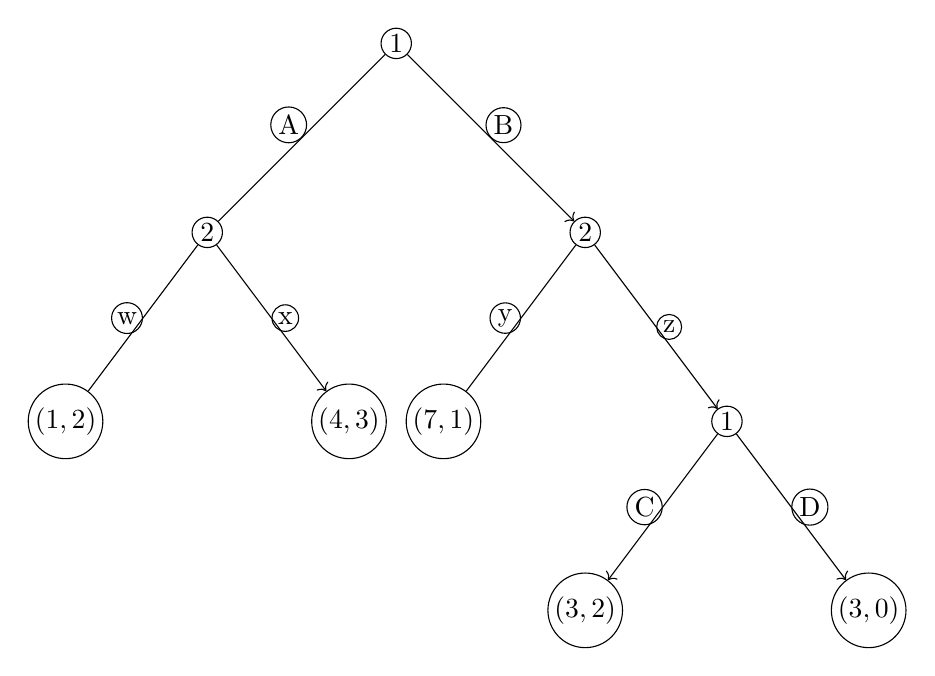
\begin{tikzpicture}[scale=1.2, every node/.style={draw, circle, inner sep=1pt}]
        \node (A) at (0,0) {1};
        \node (B) at (-2,-2) {2};
        \node (C) at (2,-2) {2};
        \node (D) at (-3.5,-4) {$(1,2)$};
        \node (E) at (-0.5,-4) {$(4,3)$};
        \node (F) at (0.5,-4) {$(7,1)$};
        \node (G) at (3.5,-4) {1};
        \node (L) at (2,-6) {$(3,2)$};
        \node (M) at (5,-6) {$(3,0)$};

        \draw (A) -- (B) node[midway, above left] {A};
        \draw[->] (A) -- (C) node[midway, above right] {B};
        \draw (B) -- (D) node[midway, left] {w};
        \draw[->] (B) -- (E) node[midway, right] {x};
        \draw (C) -- (F) node[midway, left] {y};
        \draw[->] (C) -- (G) node[midway, right] {z};
        \draw[->] (G) -- (L) node[midway, left] {C};
        \draw[->] (G) -- (M) node[midway, right] {D};
    \end{tikzpicture}
\end{center}

\begin{enumerate}
    \item[(a)] Write down the strategic form and find all Nash equilibria. For each equilibrium, find the equilibrium outcome. (Be sure you understand the difference.)
    \begin{solution}
    Strategic Form:
    \begin{table}[H]
        \centering
        \begin{tabular}{|c|c|l|l|l|} \hline 
 & wy&wz &xy &xz\\ \hline 
AC& 1,2& 1,2& 4,\textbf{3}&\textbf{4},\textbf{3}\\ \hline 
AD& 1,2&  1,2& 4,\textbf{3}&\textbf{4},\textbf{3}\\ \hline
BC& \textbf{7},1& \textbf{3},\textbf{2}& 7,1&3,\textbf{2}\\\hline
BD& \textbf{7},\textbf{1}& \textbf{3},0& \textbf{7},\textbf{1}&3,0\\\hline\end{tabular}
        \caption{Strategic Form}
    \end{table}
    From best response method in table above:
    \[\boxed{s = (AC, xz) \to O(s) = (A,x)} \]
    \[\boxed{s = (AD, xz) \to O(s) = (A,x)}\]
    \[\boxed{s = (BC, wz) \to O(s) = (B,z ,C)}\]
    \[\boxed{s = (BD, wy) \to O(s) = (B,y)}\]
    \[\boxed{s = (BD, xy) \to O(s) = (B,y)}\]
        \end{solution}
    \item[(b)] Find all subgame-perfect Nash equilibria. For each equilibrium, provide the equilibrium outcome.
    \begin{solution}
    \begin{table}[H]
        \centering
        \begin{tabular}{c|cl}
 &Optimal action  &Optimal action  \\
             Subgame 1 (1, C,D)&  C&D\\
             Subgame 2 (2, w,x,y,x)& 
         xz&xy\\
 Subgame 3 (1, A,B)& A&B\\\end{tabular}
        \caption{Finding SPNE}
    \end{table}
        From the tree and the table above, we see that the SPNE are 
        \[\boxed{ s= \{(AC, xz), (BD, xy)\}}\]
        \[\boxed{O(s_1) = (A,x)}, \quad \boxed{O(s_2) = (B, y)}\]
    \end{solution}
    \item[(c)] How do your answers to parts (a) and (b) compare? Please explain the difference, if any.
    \begin{solution}
        There are strictly less SPNE than there are Nash Equilibria. The interesting thing to note is that in no strategy which results in player one playing twice is a SPNE. That is, player two knows it is not optimal for her to let player one go again. 
    \end{solution}
\end{enumerate}

\section*{Problem 2}
Consider the ultimatum bargaining game with two players, but now assume that the players are altruistic, in the sense that they value not only their own share of the resource but also (though to a lesser extent) the other player’s share. The following utility functions represent these preferences:

\begin{align*}
    u_1 (x_1, x_2) &= x_1 + \alpha x_2, \\
    u_2 (x_1, x_2) &= \alpha x_1 + x_2,
\end{align*}
where $\alpha \in (0,1)$. If bargaining breaks down (i.e., if player 2 rejects player 1’s offer), then the players receive default shares $\bar{x}_1 = \bar{x}_2 = 0$.

\begin{enumerate}
    \item[(a)] What offers will Player 2 accept?
    \begin{solution}
    Here, we assume the total resources are $1$ (normalize if not). 
    
        If player $2$ rejects, then he gets $0$ utility. Let $x_1 \in [0,1].$ Then since $\alpha \in (0,1),$ we have that
        \[u_2(x_1, x_2) = \alpha x_1 + (1-x_1) = 1 + x_1(\alpha -1) >0,\] and so player $2$ will accept no matter what. 
    \end{solution}
    \item[(b)] What is the subgame-perfect Nash equilibrium?
    \begin{solution}
        Since player $2$ always accepts, the subgame-perfect equilibria will arise when player $1$ chooses his best possible option. That is, when $u_1(x_1, x_2)$ is maximized:
        \[u_1(x_1 + x_2) = x_1 + \alpha(1 - x_1) \implies \hat{x}_1 = 1,\] and so the subgame perfect Nash Equilibrium is simply 
        \[\boxed{s = (x_1 = 1, \text{Accept})}\]
    \end{solution}
    \item[(c)] What is the equilibrium outcome?
    \begin{solution}
        From above, 
        \[\boxed{O(s) = (1, 0)}\]
    \end{solution}
\end{enumerate}

\section*{Problem 3}
Two people select a policy among three alternatives, $X$, $Y$, and $Z$, by alternately vetoing policies until only one remains: first, person 1 vetoes a policy, following which person 2 vetoes one of the two policies that remain. Suppose person 1 strictly prefers $X$ to $Y$ to $Z$, whereas person 2 strictly prefers $Z$ to $Y$ to $X$.

\begin{enumerate}
    \item[(a)] Model this situation as an extensive game with perfect information and ordinal preferences. Draw a picture.
    \begin{solution}
    Game tree:
    \[
        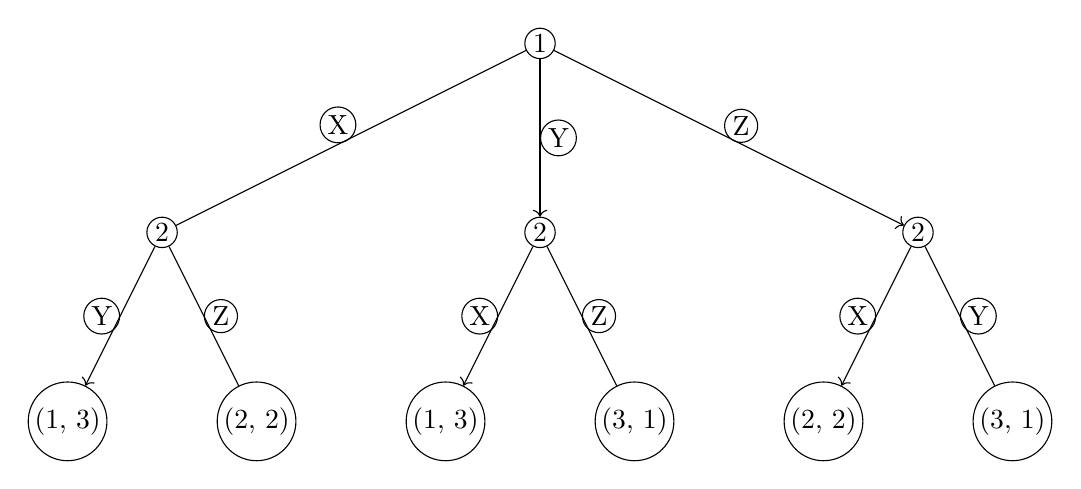
\begin{tikzpicture}[scale=1.2, every node/.style={draw, circle, inner sep=1pt}]
        \node (A) at (0,0) {1};
        
        \node (B) at (-4,-2) {2};
        \node (C) at (0,-2) {2};
        \node (D) at (4, -2) {2};
        
        \node (E) at (-5,-4) {(1, 3)};
        \node (F) at (-3,-4) {(2, 2)};

        \node (G) at (-1,-4) {(1, 3)};
        \node (H) at (1,-4) {(3, 1)};

        \node (I) at (3,-4) {(2, 2)};
        \node (J) at (5,-4) {(3, 1)};

        \draw (A) -- (B) node[midway, above left] {X};
        \draw (A) -- (C)[->] node[midway, right] {Y};
        \draw (A) -- (D)[->] node[midway, above right] {Z};

        \draw (B) -- (E)[->] node[midway, left] {Y};
        \draw (B) -- (F) node[midway, right] {Z};

        \draw (C) -- (G)[->] node[midway, left] {X};
        \draw (C) -- (H) node[midway, right] {Z};

        \draw (D) -- (I)[->] node[midway, left] {X};
        \draw (D) -- (J) node[midway, right] {Y};
    \end{tikzpicture}\]
    \end{solution}
    \item[(b)] For each of the two players, list all available strategies.
    \begin{solution}
        \[\boxed{S_1 = \begin{bmatrix}
            X\\Y\\Z
        \end{bmatrix}}\]
        \[\boxed{S_2 = \begin{bmatrix}
            YXX & YXY & YZX & YZY & ZXX & ZXY & ZZX & ZZY
        \end{bmatrix}}\]
    \end{solution}
    \item[(c)] Construct the strategic form of this game and find all Nash equilibria.
    \begin{solution}
        \begin{table}[H]
        \centering
        \begin{tabular}{|c|c|l|l|l|l|l|l|l|l} \hline 
  & YXX & YXY & YZX & YZY & ZXX & ZXY & ZZX &ZZY \\\hline 
X & 1,\textbf{3} & 1,\textbf{3} & 1,\textbf{3} & 1,\textbf{3} & \textbf{2},2 & 2,2 & 2,2 & 2,2 
    \\\hline 
Y & 1,\textbf{3} & 1,\textbf{3} & \textbf{3},1 & \textbf{3},1 & 1,\textbf{3} & 1,\textbf{3} & \textbf{3},1 &  \textbf{3},1
    \\\hline 
Z & \textbf{2},\textbf{2} & \textbf{3},1 & 2,\textbf{2} &\textbf{3},1 &\textbf{2},\textbf{2} &\textbf{3},1 & 2,\textbf{2} & \textbf{3},1
    \\\hline 
\end{tabular}
        \caption{Strategic Form}
    \end{table}
From best response method:
\[\boxed{s = (Z, YXX) \mapsto O(s) = (Z,X)}\]
\[\boxed{s = (Z, ZXX) \mapsto O(s) = (Z,X)}\]
    \end{solution}
    \item[(d)] Find all subgame-perfect Nash equilibria.
\begin{solution}
    \begin{table}[H]
        \centering
        \begin{tabular}{cl}
                                &Optimal action    \\
             Subgame 1 (2, $S_2$)&  YXX\\
             Subgame 2 (2, $S_1$)& Z
             \\\end{tabular}
        \caption{Finding SPNE}
    \end{table}
    From the arrows in the tree and the table above, we see that \[\boxed{s = (Z, YXX) \implies O(s) = (Z,X)}\] is the unique SPNE and the unique outcome.
\end{solution}
    \item[(e)] Does the game have any Nash equilibria that are not subgame-perfect Nash equilibria? Is any outcome of a Nash equilibrium not the outcome of some subgame-perfect Nash equilibrium?
    \begin{solution}
        The game has two Nash Equilibrium but only one SPNE. However, the game only has a single NE outcome, which corresponds of course to the SPNE outcome.
    \end{solution}
\end{enumerate}


















\end{document}